


\begin{table*}
\caption{Performance (\emph{LFW} Restricted View 2) of the family of biologically-inspired models and blends thereof.} 

\centering
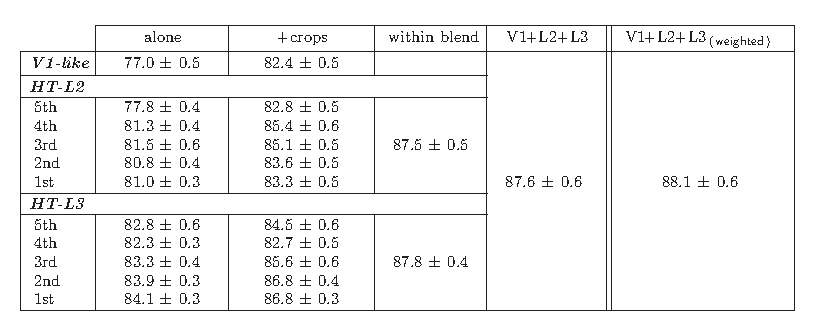
\includegraphics{tables/grand_performance_table_baked.pdf}

\label{tab:grand_performance_table}
\end{table*}





\subsection{High-throughput screening with \emph{LFW} View 1}

Fig. \ref{fig:ht_process} shows the results of high-throughput screening to select
model instantiations that are well-suited to the \emph{LFW} verification task.
For each model class, a multitude of models were randomly generated and
evaluated on the \emph{LFW} view 1 set, and the best five were selected for
further analysis.


\subsection{Performance on \emph{LFW} Restricted View 2}

Performance of individual models and model blends are shown in Table
\ref{tab:grand_performance_table}.  Performance ranging from 77.1 \% for the
simplest \emph{V1-like} model to 88.1\% for the largest blend were observed.  Taken
together, these results show that state-of-the-art level performance is possible
within the model family, and there exist multiple paths (e.g. based purely
on \emph{V1-like} models, and based on high-throughput, multi-layer models) to
achieving high levels of performance.  Fig. \ref{fig:roc_curves} shows
receiver-operator characteristic (ROC) curves for each of these models.

Interestingly, the inclusion of a single additional comparison function to the
\emph{V1-like} model blend described in \cite{pinto:cvpr09} brings an additional
3\% performance, placing it close to the last reported best performance on this
set, even without extensive blending.  Furthermore, we see that individual
\emph{HT-L3} models also perform surprisingly well --- coming to within a few percent correct of
the previous state-of-the-art.

A major advantage of our high-throughput approach is that it produces not one,
but a diversity of models, and this situation is ideally suited to kernel
blending approaches.  Once blending is added, especially when coupled with an
intelligent algorithm for weighting blended kernels, several different blends
achieved performance exceeding previously reported state-of-the-art values (see Figure \ref{fig:table_soa}).  ROC 
curves for various blend groupings are shown in Fig. \ref{fig:roc_curves}.

\begin{figure*}[ht]
\centering 
\subfigure[\small{within-model-class blends}]{
  \includegraphics[scale=0.9]{figures/within_roc.pdf}
  \label{fig:within_rocs}
} 
\subfigure[\small{across-model-class blends}]{
  \includegraphics[scale=0.9]{figures/mega_blend_roc.pdf}
  \label{fig:megablend_rocs}
}
\subfigure[\small{comparison with literature}]{
    \begin{tabular}{|c||c|c|c|c|}
\hline
%Reference & Kumar et al. ICCV09 \cite{kumar:iccv09} & Wolf et al. ACCV09 \cite{wolf:accv09} & Cao et al. CVPR10 \cite{cao2010face} & This paper \\
 & Kumar et al. & Wolf et al. & Cao et al. & \\
Reference & ICCV09 \cite{kumar:iccv09} & ACCV09 \cite{wolf:accv09} & CVPR10 \cite{cao2010face} & This paper\\
\hline\hline
Mean classification error & 14.7\%$\pm$1.2 & 13.2\%$\pm$0.3 & 15.5\%$\pm$0.5 & \bf{11.9\%$\pm$0.6} \\
\hline
\end{tabular}
\label{fig:table_soa}
}

\caption[]{{\bf ROC curves for various model sub-families on \emph{LFW}
    Restricted View 2.} Curves for \cite{wolf:accv09}, \cite{kumar:iccv09} and \cite{cao2010face} 
  are plotted in \ref{fig:megablend_rocs} for reference.  Plots are zoomed-in to
  facilitate comparison.}
\label{fig:roc_curves}
\end{figure*}


\begin{figure*}[ht]
  \centering \subfigure[Misses]{ 
    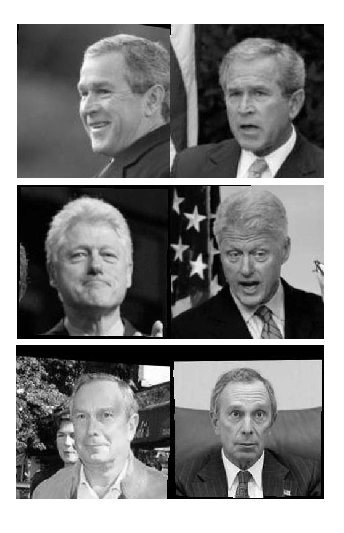
\includegraphics[scale=0.8]{figures/misses.pdf}
    \label{fig:misses}
  } \subfigure[False Positives]{
    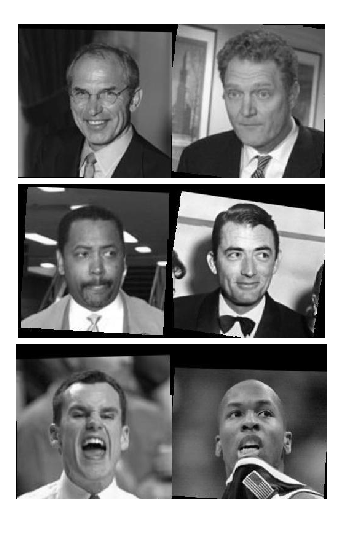
\includegraphics[scale=0.8]{figures/false_positives.pdf}
    \label{fig:false_positives}
  }
  \caption[]{{\bf Examples of common errors across models.} Misses tend to be
    dominated by differences in view, while false positives frequently occur when
    different individuals share a common view or expression. }
  \label{fig:error_examples}
\end{figure*}



\subsection{Analysis of Errors}

To understand better where room for improvement lies, we examined the error
trials (misses and false alarms) produced by each model for quantitative and
qualitative trends.  To determine whether different models were primarily making
the same or different errors, we segregated the responses of the \emph{V1-like}
and \emph{HT-L3} models (rescaled-crop augmented variants, see Methods) into
four categories: hits, misses, false positives, and correct rejections.  We then
computed the fraction of errors that these two models held in common and found
84.3\% of false positives were the same across the two models, and that
87.3\% of misses were missed by both models.  This high level of consistency
between error cases across the two models led us to ask whether a subset of
``hard'' images within the larger \emph{LFW} set could be driving errors and
capping performance.

Fig. \ref{fig:error_examples} shows examples of misses and false positives
held in common for both models.  While developing a quantitative framework
within which to analyze these errors is beyond the scope of this paper, several
patterns are evident, even upon casual inspection.  First, misses are dominated
by situations where the individual-to-be-matched is seen in non-frontal view in
at least one of the images.  Second, false positives appear to occur more often
in cases where different individuals appear in a very similar view, or with a
similar expression.


\subsection{Analysis of Tolerance to Variation, Using Synthetic Faces}

% -------------------------------------
%  Variation level figure
% -------------------------------------

\begin{figure}[ht]
    \centering
    \includegraphics[scale=0.8]{figures/eight_faces_naturalbg_variation_v1like_a_plus.pdf}
    \caption[]{{\bf Model performance on synthetic faces as a function of level of variation}}
	\label{fig:perf_variation_levels}
\end{figure}

\subsubsection{Performance as a function of variation level}

The synthetic face evaluation sets used here provide us with the ability to parametrically control the level of rotation, position and scale variation that our models are required to tolerate.  Figure \ref{fig:perf_variation_levels} shows the performance the best models from each model class (V1-like, HT-L2, HT-L3) as a function of (composite) variation level for an eight-way face classification task.


\subsubsection{Effect of number of faces to be discriminated}

To further explore the behavior of our models with a controlled stimulus, we examined model
performance as a function of the number of faces to be discriminated.  In particular, we
considered cases with two, four, six, and eight faces.  Performance, grouped by model is shown
in Figure \ref{fig:nfaces_by_model}, and is shown grouped by variation level in 
Figure \ref{fig:nfaces_by_variation}.  Predictably, absolute performance level is depressed as a larger
number of faces is considered, as is the chance performance level (dotted line). Interestingly, the
rate at which performance falls off varies between models as a function of both number of faces
to be discriminated, and as a function of variation level.  The stability of the performance of the 
largest/deepest model --- HT-L3-1st --- is most pronounced when large number of faces and large amounts of variation 
are considered.  Differences between models are far less pronounced with smaller numbers of
faces and lesser degrees of variation.
 
% -------------------------------------
%  N Faces Figure 2
% -------------------------------------

\begin{figure*}[ht!]
\centering 
\subfigure[\small{V1-like}]{
  \includegraphics[scale=0.65]{figures/nfaces_variation_NaturalBg_v1like_a_plus.pdf}
  \label{fig:nfaces_v1like}
} 
\subfigure[\small{HT-L2-1st}]{
  \includegraphics[scale=0.65]{figures/nfaces_variation_NaturalBg_ht1_1_l2_1st.pdf}
  \label{fig:nfaces_l2}
} 
\subfigure[\small{HT-L3-1st}]{
  \includegraphics[scale=0.65]{figures/nfaces_variation_NaturalBg_ht1_1_l3_1st.pdf}
  \label{fig:nfaces_l3}
}
\caption[]{{\bf Effect of number of synthetic faces to be discriminated, sorted by model}}
\label{fig:nfaces_by_model}
\end{figure*}

% -------------------------------------
%  N Faces Figure
% -------------------------------------

\begin{figure*}[ht]
\centering 
% \subfigure[\small{no variation}]{
%   \includegraphics[scale=0.6]{figures/nfaces_variation0_by_model.pdf}
%   \label{fig:nfaces_var0}
% } 
\subfigure[\small{variation level 2}]{
  \includegraphics[scale=0.7]{figures/nfaces_variation2_by_model.pdf}
  \label{fig:nfaces_var2}
} 
\subfigure[\small{variation level 4}]{
  \includegraphics[scale=0.7]{figures/nfaces_variation4_by_model.pdf}
  \label{fig:nfaces_var4}
}
\subfigure[\small{variation level 6}]{
  \includegraphics[scale=0.7]{figures/nfaces_variation6_by_model.pdf}
  \label{fig:nfaces_var6}
}

\caption[]{{\bf Effect of number of synthetic faces to be discriminated, sorted by variation level.} Note that the performance was 100\% in all cases for the zero variation condition (data not shown).}
\label{fig:nfaces_by_variation}
\end{figure*}


\subsubsection{Effect of background}

To explore the role of background variation, we evaluated model performance with four different background conditions: no background, white-noise background, phase-scrambled natural backgrounds (i.e. approx. 1/f noise), and natural backgrounds.  Performance as a function of background and variation level is shown Figure \ref{fig:perf_bg_variation}.  Choice of background was found to have a profound effect on model performance.  In the absence of a background, the performance for most models remained high, even at relatively high levels of variation in view, position, and scale (e.g. greater than 90\% performance at variation level 4 for the HT-L3-1st and V1-like models).  However, the inclusion of any background resulted in a precipitous drop-off in performance for all models, except for the HT-L3-1st model, whose performance degraded gradually.  In general, progressively more realistic backgrounds proved increasingly difficult for all models.

% -------------------------------------
%  Effect of Background Figure
% -------------------------------------

\begin{figure*}[ht]
\centering 
% \subfigure[\small{no variation}]{
%   \includegraphics[scale=0.45]{figures/bg_variation0_by_model.pdf}
%   \label{fig:bg_var0}
% } 
\subfigure[\small{variation level 2}]{
  \includegraphics[scale=0.55]{figures/bg_variation2_by_model.pdf}
  \label{fig:bg_var2}
} 
\subfigure[\small{variation level 4}]{
  \includegraphics[scale=0.55]{figures/bg_variation4_by_model.pdf}
  \label{fig:bg_var4}
}
\subfigure[\small{variation level 6}]{
  \includegraphics[scale=0.55]{figures/bg_variation6_by_model.pdf}
  \label{fig:bg_var6}
}

\caption[]{{\bf Effect of background type on performance with synthetic faces.} Note that the performance was 100\% in all cases for the zero variation condition (data not shown).}
\label{fig:perf_bg_variation}
\end{figure*}



% \subsection{Performance of models on a synthetic variation ``litmus test'' set}
